\section{Calibrazione}
\subsection{Taratura}
	Per effettare la taratra della nostra strumentazione
	abbiamo montato la lampada al mercurio,
	dopodiché abbiamo effettato n procedimento molto
	simile a qella della \sezione{sez:calib_a}.
	si é infatti
	rimosso il reticolo ed allineato la
	fenditura di uscita della sorgente,la fessura della slitta
	ed il reticolo a croce del telescopio di osservazione.
	Per effettuare tale allineamento sono state impiegate 
	le viti del piatto per effettare allineamento fine.
	Abbiamo assunto la lettura del goniometro
	$\alpha_0$ quale zero di riferimento per le successive misure.
	Essendo tale misura basilare per le osservazioni successive
	abbiamo iterato tale misurazione più volte
	ottenendo $\alpha_{ref}=	\pm		$.
	abbiamo reinserito il reticolo ponendolo in 
	maniera che esso descrivesse n angolo $\sim \ang{60}$
	tra normale e fascio incidente e che il reticolo sia allineato 
	con le lenti dei telescopi.
\subsection{Misrazione passo reticolare}
	Per effettuare la calibrazione spettrale abbiamo 
	osservato la posizione angolare per la riflessione 
	e per la riga di emissione principale del mercurio al 
	primo ordine di diffrazione $\lambda =546.074\text{ [nm]}$,
	ottenendo rispettivamente $\alpha_0=	\pm		\qquad\text{e}\qquad	\alpha_i=	\pm		$.
	Essendo nota
	\smallskip
	\begin{equation}\label{eq:passo_reticolo}
	d(sin \alpha_i - sin \alpha_d) = m \lambda\qquad \theta_i=\frac{1}{2}(\pi- \alpha_0)\qquad \alpha_d=(\pi- \theta_1-\alpha_i)
	\end{equation}
	l'\equazione{eq:passo_reticolo},dove gli angoli siano presi come in 
	\bigskip
	\begin{figure} [!h]
		\centering
		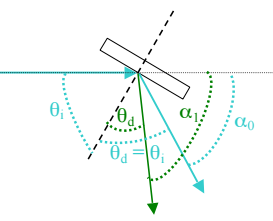
\includegraphics[width=0.9\textwidth]{./angoli.png}
		\caption{Schema della convenzioni degli angoli impiegata.}
		\label{fig:angoli}
	\end{figure}
	\smallskip
	\figura{fig:angoli},
	possiamo ricavare il passo reticolare $d$.
	Dalle misure effettate otteniamo $d=	\pm 	[mm]$

\section{Misrura $\lambda$ delle righe di emissione di na lampada al
	idrogeno}
	Per qeste misre abbiamo posto come sorgente na lampada all'idrogeno;
	dopo aver aspettato qalche minto perchè la lampada termalizzasse 
	dopodiché abbiamo allineato la lampada con la fenditra 
	posta sl telescopio di raccolta.
	Si sono misate le posizioni angolari delle varie righe osservabili
	essendo valida l'\equazione{eq:passo_reticolo}
	si ricavano le $\lambda$  riportate in 
	\smallskip
	\begin{table}[hb]
	\centering
		\begin{tabular}{|c|c|c|c|}
		\hline
		riga & ordine & $\alpha _{i}$ & $\lambda \text{ [nm]}$ \\
		\hline
		doppietto viola (intensa) & $ 1 $ &$77.66 \pm 0.05 $ & $89.1 \pm 0.1$\\
		\hline
		linea azzurra (intensa) & $ 1$ & $81.63 \pm 0.05 $ &$93.1 \pm 0.1$\\
		\hline
		doppietto verde & $ 1$ & $85.25 \pm 0.05 $ &$96.7 \pm 0.1$\\
		\hline
		linea rossa (debole) &$ 1$ & $90.66 \pm 0.05 $&$102.1 \pm 0.1$ \\
		\hline
		linea rossa (intensa) &$1$ & $93.50 \pm 0.05$ &$104.9 \pm 0.1$\\
		\hline
		doppietto viola (intensa) & $ 2$ & $ 108.42 \pm 0.05 $ &$119.9 \pm 0.1$\\
		\hline
		linea azzurra (intensa) & $ 2 $ & $115.53 \pm 0.05 $ &$127.0 \pm 0.1$\\
		\hline
		doppietto verde & $ 2$ & $122.38 \pm 0.05 $&$133.8 \pm 0.1$ \\
		\hline
		\end{tabular}
		\caption{misure delle posizioni angolari delle righe di emissione di lampada idrogeno; tali angoli sono dati rispetto ad $\alpha_{ref}$.
		Per le $\lambda$ è stata impiegata l'\equazione{eq:passo_reticolo} per n $d= 	\pm		$.}
		\label{tab:hydrogen}
	\end{table}
	\smallskip
	\tabella{tab:hydrogen}
\section{Determinazione della costante di Rydberg R}
	Impiagando l'\equazione{eq:ryd}
	\smallskip
	\begin{equation}\label{eq:ryd}
	\frac{1}{\lambda}=R(\frac{1}{({n_1}^2)}-\frac{1}{({n_2}^2)})
	\end{equation}
	\smallskip
	possiamo andare a legare la lunghezza d'onda $\lambda$
	associata alla transizione dalle righe di balmer e conoscendo 
	i relativi $n_1$ e $n_2$
	si ottengono gli $R_i$ riportati in \tabella{tab:R}.
		\smallskip
	\begin{table}[hb]
	\centering
		\begin{tabular}{|c|}
		\hline
		$ R [m^{-1}]$ \\
		\hline
		$89.1 \pm 0.1$\\
		\hline
		$93.1 \pm 0.1$\\
		\hline
		$96.7 \pm 0.1$\\
		\hline
		\end{tabular}
		\caption{$R$ misrate delle righe di emissione di lampada idrogeno.}
		\label{tab:R}
	\end{table}
	\smallskip
	Dai dati ottenti facendo n fit \bigskip
	VA FATTO FIT
	\bigskip si ottiene
	$R= 	\pm		[m^{-1}]$.
\section{Misra della risolzione dell'interferometro}
	Per effettare la misra della sensibilità dello
	spettroscopio abbiamo montato come sorgente la 
	lampada al sodio,abbiamo aspettato alcni minti
	per far termalizzare  la lampada.
	Spostato la posizione del telescopio
	di ossevazione Si sono misrate le loro posizioni angolari,
	corrispondenti  doppietto giallo
	del sodio, ottenendo $$\alpha_1=		\pm \ang{0.05}
	\text{ e }\alpha_2=		\pm \ang{0.05}$$
	impiegando l'\equazione{eq:passo_reticolo} si ottiene 
	\smallskip
	$$\lambda_1= 		\pm		\text{ [nm] e } \lambda_2= 		\pm		\text{ [nm]}$$
	Possiamo osservare che tali misure risultano ??in accordo?? con 
	la misra effettata con l'apparato in \sezione{sez:str_a}.
	Essendo nota $\Delta 	\lambda=0.6 \text{ [nm]}$
	$$HO-DBBIO-SE-NOMINALE-O-VA-MISRATO$$
	,ovvero la separazione delle de
	righe del doppietto in esame, e dalla conoscenza di 
	$\Delta \alpha= \alpha_2 -\alpha_1 =$
	possiamo effettare la vera e propria stima della
	risolzzione strmentale dal rapporto 
	$$ \frac{\Delta \lambda}{\Delta \alpha}= 	\pm			\text{ [nm]}$$
	Essendo la separazione del doppietto della riga di emissiame gialla
	della lampada maggiore della nostra risolzione strmentale.
	Pertanto la separazione del doppietto rislta osservabile.